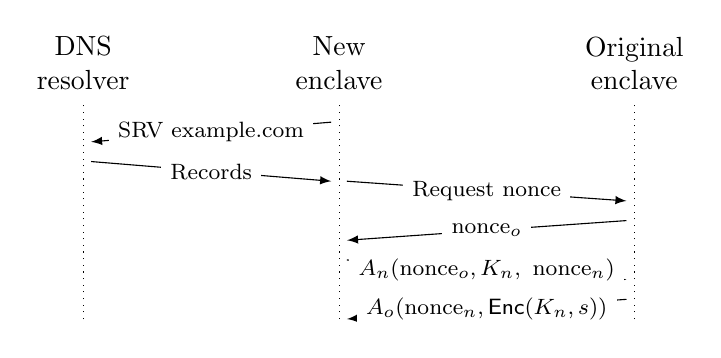
\begin{tikzpicture}[node distance=20pt]

  \def\dnsright{0.1}
  \def\newleft{3.15}
  \def\newright{3.35}
  \def\origleft{6.9}

  %               x,    y      x,    y
  \draw [dotted] (0,    0) -- (0,    2.75);
  \draw [dotted] (3.25, 0) -- (3.25, 2.75);
  \draw [dotted] (7,    0) -- (7,    2.75);

  \node [align=center] at (0,    3.25) {DNS\\resolver};
  \node [align=center] at (3.25, 3.25) {New\\enclave};
  \node [align=center] at (7,    3.25) {Original\\enclave};

  % New enclave discovers existing enclaves via DNS.
  \draw [-latex] (\newleft, 2.5) -- (\dnsright, 2.25)
        node [midway, align=center, fill=white]
        {\footnotesize SRV example.com};
  \draw [-latex] (\dnsright, 2) -- (\newleft, 1.75)
        node [midway, align=center, fill=white]
        {\footnotesize Records};

  \draw [-latex] (\newright, 1.75) -- (\origleft, 1.5)
        node [midway, fill=white, align=center]
        {\footnotesize Request nonce};
  \draw [-latex] (\origleft, 1.25) -- (\newright, 1)
        node [midway, fill=white, align=center]
        {\footnotesize $\textrm{nonce}_o$};

  % New enclave asks for keys.
  \draw [-latex] (\newright, 0.75) -- (\origleft, 0.5)
        node [midway, fill=white, align=center]
        {\footnotesize $A_{n}(\textrm{nonce}_o, K_n, \ \textrm{nonce}_n$)};

  \draw [-latex] (\origleft, 0.25) -- (\newright, 0)
        node [midway, fill=white, align=center]
        {\footnotesize $A_{o}(\textrm{nonce}_n, \textsf{Enc}(K_n, s))$};

\end{tikzpicture}
